


% Header, overrides base

    % Make sure that the sphinx doc style knows who it inherits from.
    \def\sphinxdocclass{article}

    % Declare the document class
    \documentclass[letterpaper,10pt,english]{/usr/share/sphinx/texinputs/sphinxhowto}

    % Imports
    \usepackage[utf8]{inputenc}
    \DeclareUnicodeCharacter{00A0}{\\nobreakspace}
    \usepackage[T1]{fontenc}
    \usepackage{babel}
    \usepackage{times}
    \usepackage{import}
    \usepackage[Bjarne]{/usr/share/sphinx/texinputs/fncychap}
    \usepackage{longtable}
    \usepackage{/usr/share/sphinx/texinputs/sphinx}
    \usepackage{multirow}

    \usepackage{amsmath}
    \usepackage{amssymb}
    \usepackage{ucs}
    \usepackage{enumerate}

    % Used to make the Input/Output rules follow around the contents.
    \usepackage{needspace}

    % Pygments requirements
    \usepackage{fancyvrb}
    \usepackage{color}
    % ansi colors additions
    \definecolor{darkgreen}{rgb}{.12,.54,.11}
    \definecolor{lightgray}{gray}{.95}
    \definecolor{brown}{rgb}{0.54,0.27,0.07}
    \definecolor{purple}{rgb}{0.5,0.0,0.5}
    \definecolor{darkgray}{gray}{0.25}
    \definecolor{lightred}{rgb}{1.0,0.39,0.28}
    \definecolor{lightgreen}{rgb}{0.48,0.99,0.0}
    \definecolor{lightblue}{rgb}{0.53,0.81,0.92}
    \definecolor{lightpurple}{rgb}{0.87,0.63,0.87}
    \definecolor{lightcyan}{rgb}{0.5,1.0,0.83}

    % Needed to box output/input
    \usepackage{tikz}
        \usetikzlibrary{calc,arrows,shadows}
    \usepackage[framemethod=tikz]{mdframed}

    \usepackage{alltt}

    % Used to load and display graphics
    \usepackage{graphicx}
    \graphicspath{ {figs/} }
    \usepackage[Export]{adjustbox} % To resize

    % used so that images for notebooks which have spaces in the name can still be included
    \usepackage{grffile}


    % For formatting output while also word wrapping.
    \usepackage{listings}
    \lstset{breaklines=true}
    \lstset{basicstyle=\small\ttfamily}
    \def\smaller{\fontsize{9.5pt}{9.5pt}\selectfont}

    %Pygments definitions
    
\makeatletter
\def\PY@reset{\let\PY@it=\relax \let\PY@bf=\relax%
    \let\PY@ul=\relax \let\PY@tc=\relax%
    \let\PY@bc=\relax \let\PY@ff=\relax}
\def\PY@tok#1{\csname PY@tok@#1\endcsname}
\def\PY@toks#1+{\ifx\relax#1\empty\else%
    \PY@tok{#1}\expandafter\PY@toks\fi}
\def\PY@do#1{\PY@bc{\PY@tc{\PY@ul{%
    \PY@it{\PY@bf{\PY@ff{#1}}}}}}}
\def\PY#1#2{\PY@reset\PY@toks#1+\relax+\PY@do{#2}}

\expandafter\def\csname PY@tok@gd\endcsname{\def\PY@tc##1{\textcolor[rgb]{0.63,0.00,0.00}{##1}}}
\expandafter\def\csname PY@tok@gu\endcsname{\let\PY@bf=\textbf\def\PY@tc##1{\textcolor[rgb]{0.50,0.00,0.50}{##1}}}
\expandafter\def\csname PY@tok@gt\endcsname{\def\PY@tc##1{\textcolor[rgb]{0.00,0.27,0.87}{##1}}}
\expandafter\def\csname PY@tok@gs\endcsname{\let\PY@bf=\textbf}
\expandafter\def\csname PY@tok@gr\endcsname{\def\PY@tc##1{\textcolor[rgb]{1.00,0.00,0.00}{##1}}}
\expandafter\def\csname PY@tok@cm\endcsname{\let\PY@it=\textit\def\PY@tc##1{\textcolor[rgb]{0.25,0.50,0.50}{##1}}}
\expandafter\def\csname PY@tok@vg\endcsname{\def\PY@tc##1{\textcolor[rgb]{0.10,0.09,0.49}{##1}}}
\expandafter\def\csname PY@tok@m\endcsname{\def\PY@tc##1{\textcolor[rgb]{0.40,0.40,0.40}{##1}}}
\expandafter\def\csname PY@tok@mh\endcsname{\def\PY@tc##1{\textcolor[rgb]{0.40,0.40,0.40}{##1}}}
\expandafter\def\csname PY@tok@go\endcsname{\def\PY@tc##1{\textcolor[rgb]{0.53,0.53,0.53}{##1}}}
\expandafter\def\csname PY@tok@ge\endcsname{\let\PY@it=\textit}
\expandafter\def\csname PY@tok@vc\endcsname{\def\PY@tc##1{\textcolor[rgb]{0.10,0.09,0.49}{##1}}}
\expandafter\def\csname PY@tok@il\endcsname{\def\PY@tc##1{\textcolor[rgb]{0.40,0.40,0.40}{##1}}}
\expandafter\def\csname PY@tok@cs\endcsname{\let\PY@it=\textit\def\PY@tc##1{\textcolor[rgb]{0.25,0.50,0.50}{##1}}}
\expandafter\def\csname PY@tok@cp\endcsname{\def\PY@tc##1{\textcolor[rgb]{0.74,0.48,0.00}{##1}}}
\expandafter\def\csname PY@tok@gi\endcsname{\def\PY@tc##1{\textcolor[rgb]{0.00,0.63,0.00}{##1}}}
\expandafter\def\csname PY@tok@gh\endcsname{\let\PY@bf=\textbf\def\PY@tc##1{\textcolor[rgb]{0.00,0.00,0.50}{##1}}}
\expandafter\def\csname PY@tok@ni\endcsname{\let\PY@bf=\textbf\def\PY@tc##1{\textcolor[rgb]{0.60,0.60,0.60}{##1}}}
\expandafter\def\csname PY@tok@nl\endcsname{\def\PY@tc##1{\textcolor[rgb]{0.63,0.63,0.00}{##1}}}
\expandafter\def\csname PY@tok@nn\endcsname{\let\PY@bf=\textbf\def\PY@tc##1{\textcolor[rgb]{0.00,0.00,1.00}{##1}}}
\expandafter\def\csname PY@tok@no\endcsname{\def\PY@tc##1{\textcolor[rgb]{0.53,0.00,0.00}{##1}}}
\expandafter\def\csname PY@tok@na\endcsname{\def\PY@tc##1{\textcolor[rgb]{0.49,0.56,0.16}{##1}}}
\expandafter\def\csname PY@tok@nb\endcsname{\def\PY@tc##1{\textcolor[rgb]{0.00,0.50,0.00}{##1}}}
\expandafter\def\csname PY@tok@nc\endcsname{\let\PY@bf=\textbf\def\PY@tc##1{\textcolor[rgb]{0.00,0.00,1.00}{##1}}}
\expandafter\def\csname PY@tok@nd\endcsname{\def\PY@tc##1{\textcolor[rgb]{0.67,0.13,1.00}{##1}}}
\expandafter\def\csname PY@tok@ne\endcsname{\let\PY@bf=\textbf\def\PY@tc##1{\textcolor[rgb]{0.82,0.25,0.23}{##1}}}
\expandafter\def\csname PY@tok@nf\endcsname{\def\PY@tc##1{\textcolor[rgb]{0.00,0.00,1.00}{##1}}}
\expandafter\def\csname PY@tok@si\endcsname{\let\PY@bf=\textbf\def\PY@tc##1{\textcolor[rgb]{0.73,0.40,0.53}{##1}}}
\expandafter\def\csname PY@tok@s2\endcsname{\def\PY@tc##1{\textcolor[rgb]{0.73,0.13,0.13}{##1}}}
\expandafter\def\csname PY@tok@vi\endcsname{\def\PY@tc##1{\textcolor[rgb]{0.10,0.09,0.49}{##1}}}
\expandafter\def\csname PY@tok@nt\endcsname{\let\PY@bf=\textbf\def\PY@tc##1{\textcolor[rgb]{0.00,0.50,0.00}{##1}}}
\expandafter\def\csname PY@tok@nv\endcsname{\def\PY@tc##1{\textcolor[rgb]{0.10,0.09,0.49}{##1}}}
\expandafter\def\csname PY@tok@s1\endcsname{\def\PY@tc##1{\textcolor[rgb]{0.73,0.13,0.13}{##1}}}
\expandafter\def\csname PY@tok@sh\endcsname{\def\PY@tc##1{\textcolor[rgb]{0.73,0.13,0.13}{##1}}}
\expandafter\def\csname PY@tok@sc\endcsname{\def\PY@tc##1{\textcolor[rgb]{0.73,0.13,0.13}{##1}}}
\expandafter\def\csname PY@tok@sx\endcsname{\def\PY@tc##1{\textcolor[rgb]{0.00,0.50,0.00}{##1}}}
\expandafter\def\csname PY@tok@bp\endcsname{\def\PY@tc##1{\textcolor[rgb]{0.00,0.50,0.00}{##1}}}
\expandafter\def\csname PY@tok@c1\endcsname{\let\PY@it=\textit\def\PY@tc##1{\textcolor[rgb]{0.25,0.50,0.50}{##1}}}
\expandafter\def\csname PY@tok@kc\endcsname{\let\PY@bf=\textbf\def\PY@tc##1{\textcolor[rgb]{0.00,0.50,0.00}{##1}}}
\expandafter\def\csname PY@tok@c\endcsname{\let\PY@it=\textit\def\PY@tc##1{\textcolor[rgb]{0.25,0.50,0.50}{##1}}}
\expandafter\def\csname PY@tok@mf\endcsname{\def\PY@tc##1{\textcolor[rgb]{0.40,0.40,0.40}{##1}}}
\expandafter\def\csname PY@tok@err\endcsname{\def\PY@bc##1{\setlength{\fboxsep}{0pt}\fcolorbox[rgb]{1.00,0.00,0.00}{1,1,1}{\strut ##1}}}
\expandafter\def\csname PY@tok@kd\endcsname{\let\PY@bf=\textbf\def\PY@tc##1{\textcolor[rgb]{0.00,0.50,0.00}{##1}}}
\expandafter\def\csname PY@tok@ss\endcsname{\def\PY@tc##1{\textcolor[rgb]{0.10,0.09,0.49}{##1}}}
\expandafter\def\csname PY@tok@sr\endcsname{\def\PY@tc##1{\textcolor[rgb]{0.73,0.40,0.53}{##1}}}
\expandafter\def\csname PY@tok@mo\endcsname{\def\PY@tc##1{\textcolor[rgb]{0.40,0.40,0.40}{##1}}}
\expandafter\def\csname PY@tok@kn\endcsname{\let\PY@bf=\textbf\def\PY@tc##1{\textcolor[rgb]{0.00,0.50,0.00}{##1}}}
\expandafter\def\csname PY@tok@mi\endcsname{\def\PY@tc##1{\textcolor[rgb]{0.40,0.40,0.40}{##1}}}
\expandafter\def\csname PY@tok@gp\endcsname{\let\PY@bf=\textbf\def\PY@tc##1{\textcolor[rgb]{0.00,0.00,0.50}{##1}}}
\expandafter\def\csname PY@tok@o\endcsname{\def\PY@tc##1{\textcolor[rgb]{0.40,0.40,0.40}{##1}}}
\expandafter\def\csname PY@tok@kr\endcsname{\let\PY@bf=\textbf\def\PY@tc##1{\textcolor[rgb]{0.00,0.50,0.00}{##1}}}
\expandafter\def\csname PY@tok@s\endcsname{\def\PY@tc##1{\textcolor[rgb]{0.73,0.13,0.13}{##1}}}
\expandafter\def\csname PY@tok@kp\endcsname{\def\PY@tc##1{\textcolor[rgb]{0.00,0.50,0.00}{##1}}}
\expandafter\def\csname PY@tok@w\endcsname{\def\PY@tc##1{\textcolor[rgb]{0.73,0.73,0.73}{##1}}}
\expandafter\def\csname PY@tok@kt\endcsname{\def\PY@tc##1{\textcolor[rgb]{0.69,0.00,0.25}{##1}}}
\expandafter\def\csname PY@tok@ow\endcsname{\let\PY@bf=\textbf\def\PY@tc##1{\textcolor[rgb]{0.67,0.13,1.00}{##1}}}
\expandafter\def\csname PY@tok@sb\endcsname{\def\PY@tc##1{\textcolor[rgb]{0.73,0.13,0.13}{##1}}}
\expandafter\def\csname PY@tok@k\endcsname{\let\PY@bf=\textbf\def\PY@tc##1{\textcolor[rgb]{0.00,0.50,0.00}{##1}}}
\expandafter\def\csname PY@tok@se\endcsname{\let\PY@bf=\textbf\def\PY@tc##1{\textcolor[rgb]{0.73,0.40,0.13}{##1}}}
\expandafter\def\csname PY@tok@sd\endcsname{\let\PY@it=\textit\def\PY@tc##1{\textcolor[rgb]{0.73,0.13,0.13}{##1}}}

\def\PYZbs{\char`\\}
\def\PYZus{\char`\_}
\def\PYZob{\char`\{}
\def\PYZcb{\char`\}}
\def\PYZca{\char`\^}
\def\PYZam{\char`\&}
\def\PYZlt{\char`\<}
\def\PYZgt{\char`\>}
\def\PYZsh{\char`\#}
\def\PYZpc{\char`\%}
\def\PYZdl{\char`\$}
\def\PYZhy{\char`\-}
\def\PYZsq{\char`\'}
\def\PYZdq{\char`\"}
\def\PYZti{\char`\~}
% for compatibility with earlier versions
\def\PYZat{@}
\def\PYZlb{[}
\def\PYZrb{]}
\makeatother


    %Set pygments styles if needed...
    
        \definecolor{nbframe-border}{rgb}{0.867,0.867,0.867}
        \definecolor{nbframe-bg}{rgb}{0.969,0.969,0.969}
        \definecolor{nbframe-in-prompt}{rgb}{0.0,0.0,0.502}
        \definecolor{nbframe-out-prompt}{rgb}{0.545,0.0,0.0}

        \newenvironment{ColorVerbatim}
        {\begin{mdframed}[%
            roundcorner=1.0pt, %
            backgroundcolor=nbframe-bg, %
            userdefinedwidth=1\linewidth, %
            leftmargin=0.1\linewidth, %
            innerleftmargin=0pt, %
            innerrightmargin=0pt, %
            linecolor=nbframe-border, %
            linewidth=1pt, %
            usetwoside=false, %
            everyline=true, %
            innerlinewidth=3pt, %
            innerlinecolor=nbframe-bg, %
            middlelinewidth=1pt, %
            middlelinecolor=nbframe-bg, %
            outerlinewidth=0.5pt, %
            outerlinecolor=nbframe-border, %
            needspace=0pt
        ]}
        {\end{mdframed}}
        
        \newenvironment{InvisibleVerbatim}
        {\begin{mdframed}[leftmargin=0.1\linewidth,innerleftmargin=3pt,innerrightmargin=3pt, userdefinedwidth=1\linewidth, linewidth=0pt, linecolor=white, usetwoside=false]}
        {\end{mdframed}}

        \renewenvironment{Verbatim}[1][\unskip]
        {\begin{alltt}\smaller}
        {\end{alltt}}
    

    % Help prevent overflowing lines due to urls and other hard-to-break 
    % entities.  This doesn't catch everything...
    \sloppy

    % Document level variables
    \title{skydiving}
    \date{September 09, 2013}
    \release{}
    \author{Milad H. Mobarhan}
    \renewcommand{\releasename}{}

    % TODO: Add option for the user to specify a logo for his/her export.
    \newcommand{\sphinxlogo}{}

    % Make the index page of the document.
    \makeindex

    % Import sphinx document type specifics.
     


% Body

    % Start of the document
    \begin{document}

        
            \maketitle
        

        


        
        \section{Project 1: Simulate parachuting}

\emph{Summary.} The aim of this project is to develop a general solver
for the vertical motion of a body with quadratic air drag, verify the
solver, apply the solver to a skydiver in free fall, and finally apply
the solver to a complete parachute jump.\begin{center}\rule{3in}{0.4pt}\end{center}

\subsection{Mathematical problem}

A body moving vertically is subject to three different types of forces:
the gravity force, the drag force, and the buoyancy force. All the
mentioned forces act in the vertical direction. Newton's second law of
motion applied to the body says that the sum of these forces must equal
the mass of the body times its acceleration $a$ in the vertical
direction. Taking downward as positive direction, Newton's second law
gives us

\[ma = F_g + F_b + F_d,\]

The gravity froce is $F_g = mg$, where $m$ is the mass of the body and
$g$ is the acceleration of gravity. The uplift or buoyancy force
(``Archimedes force'') is $F_b = -\varrho g V$, where $\varrho$ is the
density of the fluid, in our case air, and $V$ is the volume of the
body. The drag force is quadratic in the velocity:

\[F_d=−\frac{1}{2}C_D\varrho A\vert v\vert v,\]

where $C_D$ is a dimensionless drag coefficient depending on the body's
shape, and A is the cross-sectional area as produced by a cut plane,
perpendicular to the motion, through the thickest part of the body.

By using $a =dv/dt$ and $m =\varrho_bV$, with $\varrho_b$ as the density
of the body, the equation of motion can be expressed as:

\[ v'(t) = -{1\over2}C_D{\varrho A\over\varrho_b V}\vert v\vert v + g\left({\varrho\over\varrho_b} - 1\right)
= -a \vert v\vert v+b\]

where $a = {1\over2}C_D{\varrho A\over\varrho_b V}$ and
$b = g\left(\frac{\varrho}{\varrho_b} -1\right)$.\begin{center}\rule{3in}{0.4pt}\end{center}

\subsection{Numerical solution method}

We introduce a mesh in time with points
$0= t_0< t_1 \cdots < t_{N_t}=T$. For simplicity, we assume constant
spacing $\Delta t$ between the mesh points: $\Delta t = t_{n}-t_{n-1}$,
$n=1,\ldots,N_t$. Let $u^n$ be the numerical approximation to the exact
solution at $t_n$.

The Crank-Nicolson method is used to solve the differential equation
numerically. This method gives a nonlinear equation in $v$ when applied
to our system, but we can use a geometric average of $\vert v\vert v$ in
time to linearize the equation of motion with quadratic drag:

\[ u^{n+1} = \frac{u^n + \Delta t b^{n+\frac{1}{2}}}{1 + \Delta t a^{n+\frac{1}{2}}\vert u^{n}\vert }\]

for $n=0,1,\ldots,N_t-1$.\begin{center}\rule{3in}{0.4pt}\end{center}

\subsection{Implementation}

In this project classes have been used for implementation. A class
\texttt{Problem} holds the definition of the physical problem, a class
\texttt{ODESolver} holds the data and methods needed to numerically
solve the problem, and a class \texttt{Visualizer} to make plots.

The \texttt{ODESolver} class is implemented as the superclass of all
numerical methods for solving ODEs. This class provide all functionality
that is commen to all numerical methods for ODEs. The
\texttt{ODESolver}class has a \texttt{advance} method which is empty in
the superclass, since the method is to be implemented by various
subclasses for various numerical schemes. The Crank-Nicolson scheme is
implemented in the \texttt{advance} method of \texttt{CNQuadratic},
where the later is a subclass of \texttt{ODESolver}.

    % Make sure that atleast 4 lines are below the HR
    \needspace{4\baselineskip}

    
        \vspace{6pt}
        \makebox[0.1\linewidth]{\smaller\hfill\tt\color{nbframe-in-prompt}In\hspace{4pt}{[}1{]}:\hspace{4pt}}\\*
        \vspace{-2.65\baselineskip}
        \begin{ColorVerbatim}
            \vspace{-0.7\baselineskip}
            \begin{Verbatim}[commandchars=\\\{\}]
\PY{k}{class} \PY{n+nc}{ODESolver}\PY{p}{(}\PY{p}{)}\PY{p}{:}
    \PY{l+s+sd}{\PYZdq{}\PYZdq{}\PYZdq{}}
\PY{l+s+sd}{    Superclass for numerical methods solving scalar ODEs}

\PY{l+s+sd}{      u\PYZsq{}(t) = f(u, t)}
\PY{l+s+sd}{    \PYZdq{}\PYZdq{}\PYZdq{}}
    \PY{k}{def} \PY{n+nf}{\PYZus{}\PYZus{}init\PYZus{}\PYZus{}}\PY{p}{(}\PY{n+nb+bp}{self}\PY{p}{,}\PY{n}{problem}\PY{p}{,} \PY{n}{u0}\PY{p}{,} \PY{n}{dt}\PY{p}{,} \PY{n}{T}\PY{p}{)}\PY{p}{:}  
        \PY{n+nb+bp}{self}\PY{o}{.}\PY{n}{problem}\PY{p}{,} \PY{n+nb+bp}{self}\PY{o}{.}\PY{n}{u0}\PY{p}{,} \PY{n+nb+bp}{self}\PY{o}{.}\PY{n}{dt}\PY{p}{,} \PY{n+nb+bp}{self}\PY{o}{.}\PY{n}{T} \PY{o}{=} \PYZbs{}
                                                \PY{n}{problem}\PY{p}{,} \PY{n}{u0}\PY{p}{,} \PY{n}{dt} \PY{p}{,}\PY{n}{T}
   
    \PY{k}{def} \PY{n+nf}{advance}\PY{p}{(}\PY{n+nb+bp}{self}\PY{p}{)}\PY{p}{:}
        \PY{l+s+sd}{\PYZdq{}\PYZdq{}\PYZdq{}Advance solution one time step.\PYZdq{}\PYZdq{}\PYZdq{}}
        \PY{k}{raise} \PY{n+ne}{NotImplementedError}
        
        
    \PY{k}{def} \PY{n+nf}{solve}\PY{p}{(}\PY{n+nb+bp}{self}\PY{p}{)}\PY{p}{:}
       \PY{l+s+sd}{\PYZdq{}\PYZdq{}\PYZdq{}}
\PY{l+s+sd}{       Advance solution in time until t \PYZlt{} T.}
\PY{l+s+sd}{       \PYZdq{}\PYZdq{}\PYZdq{}}
       \PY{n+nb+bp}{self}\PY{o}{.}\PY{n}{u} \PY{o}{=} \PY{p}{[}\PY{p}{]}
       \PY{n+nb+bp}{self}\PY{o}{.}\PY{n}{t} \PY{o}{=} \PY{p}{[}\PY{p}{]}
       
       \PY{n+nb+bp}{self}\PY{o}{.}\PY{n}{u}\PY{o}{.}\PY{n}{append}\PY{p}{(}\PY{n+nb}{float}\PY{p}{(}\PY{n+nb+bp}{self}\PY{o}{.}\PY{n}{u0}\PY{p}{)}\PY{p}{)}
       \PY{n+nb+bp}{self}\PY{o}{.}\PY{n}{t}\PY{o}{.}\PY{n}{append}\PY{p}{(}\PY{l+m+mi}{0}\PY{p}{)}
       \PY{n+nb+bp}{self}\PY{o}{.}\PY{n}{dt} \PY{o}{=} \PY{n+nb}{float}\PY{p}{(}\PY{n+nb+bp}{self}\PY{o}{.}\PY{n}{dt}\PY{p}{)}            \PY{c}{\PYZsh{} avoid integer division}
       \PY{n}{Nt} \PY{o}{=} \PY{n+nb}{int}\PY{p}{(}\PY{n+nb}{round}\PY{p}{(}\PY{n+nb+bp}{self}\PY{o}{.}\PY{n}{T}\PY{o}{/}\PY{n+nb+bp}{self}\PY{o}{.}\PY{n}{dt}\PY{p}{)}\PY{p}{)}     \PY{c}{\PYZsh{} no of time intervals}
       \PY{n+nb+bp}{self}\PY{o}{.}\PY{n}{T} \PY{o}{=} \PY{n}{Nt}\PY{o}{*}\PY{n+nb+bp}{self}\PY{o}{.}\PY{n}{dt}                 \PY{c}{\PYZsh{} adjust T to fit time step dt}
       
       \PY{n}{tNew} \PY{o}{=} \PY{l+m+mi}{0}
       \PY{k}{while} \PY{n}{tNew} \PY{o}{\PYZlt{}}\PY{o}{=} \PY{n+nb+bp}{self}\PY{o}{.}\PY{n}{T}\PY{p}{:}
           \PY{n}{uNew} \PY{o}{=} \PY{n+nb+bp}{self}\PY{o}{.}\PY{n}{advance}\PY{p}{(}\PY{p}{)}
           \PY{n+nb+bp}{self}\PY{o}{.}\PY{n}{u}\PY{o}{.}\PY{n}{append}\PY{p}{(}\PY{n}{uNew}\PY{p}{)}
           \PY{n}{tNew} \PY{o}{=} \PY{n+nb+bp}{self}\PY{o}{.}\PY{n}{t}\PY{p}{[}\PY{o}{\PYZhy{}}\PY{l+m+mi}{1}\PY{p}{]} \PY{o}{+} \PY{n+nb+bp}{self}\PY{o}{.}\PY{n}{dt}
           \PY{n+nb+bp}{self}\PY{o}{.}\PY{n}{t}\PY{o}{.}\PY{n}{append}\PY{p}{(}\PY{n}{tNew}\PY{p}{)}
           
       \PY{k}{return} \PY{n}{array}\PY{p}{(}\PY{n+nb+bp}{self}\PY{o}{.}\PY{n}{u}\PY{p}{)}\PY{p}{,} \PY{n}{array}\PY{p}{(}\PY{n+nb+bp}{self}\PY{o}{.}\PY{n}{t}\PY{p}{)}
       

\PY{k}{class} \PY{n+nc}{CNQuadratic}\PY{p}{(}\PY{n}{ODESolver}\PY{p}{)}\PY{p}{:}
    \PY{l+s+sd}{\PYZdq{}\PYZdq{}\PYZdq{}}
\PY{l+s+sd}{    Computes u(t\PYZus{}n+1) from u(t\PYZus{}n), by using a Crank\PYZhy{}Nicolson scheme with }
\PY{l+s+sd}{    geometeric average approximation,  for ODE of the type:}
\PY{l+s+sd}{        }
\PY{l+s+sd}{        u\PYZsq{}(t) = \PYZhy{}a(t)*|u(t)|u(t)+b(t).}
\PY{l+s+sd}{        }
\PY{l+s+sd}{    \PYZdq{}\PYZdq{}\PYZdq{}} 

    \PY{k}{def} \PY{n+nf}{advance}\PY{p}{(}\PY{n+nb+bp}{self}\PY{p}{)}\PY{p}{:}
        \PY{n}{u}\PY{p}{,} \PY{n}{dt}  \PY{o}{=} \PY{n+nb+bp}{self}\PY{o}{.}\PY{n}{u}\PY{p}{[}\PY{o}{\PYZhy{}}\PY{l+m+mi}{1}\PY{p}{]}\PY{p}{,} \PY{n+nb+bp}{self}\PY{o}{.}\PY{n}{dt}     
        
        \PY{n}{a} \PY{o}{=} \PY{n+nb+bp}{self}\PY{o}{.}\PY{n}{problem}\PY{o}{.}\PY{n}{a}\PY{p}{(}\PY{n+nb+bp}{self}\PY{o}{.}\PY{n}{t}\PY{p}{[}\PY{o}{\PYZhy{}}\PY{l+m+mi}{1}\PY{p}{]}\PY{o}{+}\PY{n}{dt}\PY{o}{*}\PY{l+m+mf}{0.5}\PY{p}{)}
        \PY{n}{b} \PY{o}{=} \PY{n+nb+bp}{self}\PY{o}{.}\PY{n}{problem}\PY{o}{.}\PY{n}{b}\PY{p}{(}\PY{n+nb+bp}{self}\PY{o}{.}\PY{n}{t}\PY{p}{[}\PY{o}{\PYZhy{}}\PY{l+m+mi}{1}\PY{p}{]}\PY{o}{+}\PY{n}{dt}\PY{o}{*}\PY{l+m+mf}{0.5}\PY{p}{)}
            
                
        \PY{n}{uNew} \PY{o}{=} \PY{p}{(}\PY{n}{u} \PY{o}{+} \PY{n}{dt}\PY{o}{*}\PY{n}{b}\PY{p}{)}\PY{o}{/}\PY{p}{(}\PY{l+m+mi}{1}\PY{o}{+}\PY{n}{dt}\PY{o}{*}\PY{n}{a}\PY{o}{*}\PY{n+nb}{abs}\PY{p}{(}\PY{n}{u}\PY{p}{)}\PY{p}{)}
                
        \PY{k}{return} \PY{n}{uNew}
\end{Verbatim}

            
                \vspace{-0.2\baselineskip}
            
        \end{ColorVerbatim}
    
\begin{center}\rule{3in}{0.4pt}\end{center}

\subsection{Verfication}

In order to verify the solver, the method of manufactured solutions is
used, by fitting a source term. We choose a linear solution $u(t)=ct+d$.
From the initial condition it follows that $d=u_0$. Inserting this $u$
in the ODE results in:

\[ \frac{u^{n+1}-u^{n}}{\Delta t} = - a^{n+1/2} \vert u^{n}\vert  u^{n+1} + b^{n+1/2}\]

\[ c = - a^{n+1/2} \vert ct_n+u_0\vert  (ct_{n+1}+u_0) + b^{n+1/2}\]

Any function $u(t)=ct+u_0$ is then a correct solution if we choose

\[b^{n+1/2} = c +a^{n+1/2} \vert ct_n+u_0\vert  (ct_{n+1}+u_0) \]

With this $b$ there are no restrictions on $a$ and $c$. Without the
source term, the linear function do not satisfy the equation:

\[ u^{n+1} = \frac{u^n}{1 + \Delta t a^{n+\frac{1}{2}}\vert u^{n}\vert },\]

so a linear function of $t$ does not fulfill the discrete equations
because of the geometric mean used for the quadratic drag term.

For further verification, the method of manufactured solutions, is used
to compute the convergence rate in this problem. The expected error goes
like $\Delta t^2$ because we use a centered finite difference
approximation with error $O(\Delta t^2)$ and a geometric mean
approximation with error $O(\Delta t^2)$. A nosetest is implemented for
checking that the convergence rate is correct, by using a linear
solution of type $u(t)=ct+u_0$. In this case the source term is set to

\[b^{n} = c +a^{n} \vert ct_n+u_0\vert  (ct_n+u_0) \]

to satisfy

\[ \frac{u^{n+1}-u^{n}}{\Delta t} = - a^{n} \vert u^{n}\vert  u^{n} + b^{n}.\]\subsection{Running tests}

We have implemented two nosetests, in a seperate file named
\texttt{test\_nose.py}. One of the test checks that a linear function of
$t$ is a solution of the discrete equations. The nose test checks that
this solution is reproduced to machine precision. The other test checks
that we have the correct convergence rate. Both tests can be executed by
evaluating the cell below.

    % Make sure that atleast 4 lines are below the HR
    \needspace{4\baselineskip}

    
        \vspace{6pt}
        \makebox[0.1\linewidth]{\smaller\hfill\tt\color{nbframe-in-prompt}In\hspace{4pt}{[}2{]}:\hspace{4pt}}\\*
        \vspace{-2.65\baselineskip}
        \begin{ColorVerbatim}
            \vspace{-0.7\baselineskip}
            \begin{Verbatim}[commandchars=\\\{\}]
\PY{k+kn}{import} \PY{n+nn}{subprocess}
\PY{k}{try}\PY{p}{:}
    \PY{n}{output} \PY{o}{=} \PY{n}{subprocess}\PY{o}{.}\PY{n}{check\PYZus{}output}\PY{p}{(}\PY{p}{[}\PY{l+s}{\PYZdq{}}\PY{l+s}{nosetests}\PY{l+s}{\PYZdq{}}\PY{p}{,} \PY{l+s}{\PYZdq{}}\PY{l+s}{\PYZhy{}s}\PY{l+s}{\PYZdq{}}\PY{p}{]}\PY{p}{,} \PY{n}{stderr}\PY{o}{=}\PY{n}{subprocess}\PY{o}{.}\PY{n}{STDOUT}\PY{p}{,} \PY{n}{cwd} \PY{o}{=} \PY{l+s}{\PYZdq{}}\PY{l+s}{../../src}\PY{l+s}{\PYZdq{}}\PY{p}{)}
    \PY{k}{print} \PY{n}{output}
\PY{k}{except} \PY{n}{subprocess}\PY{o}{.}\PY{n}{CalledProcessError} \PY{k}{as} \PY{n}{ex}\PY{p}{:}
    \PY{k}{print} \PY{n}{ex}\PY{o}{.}\PY{n}{output} 
\end{Verbatim}

            
                \vspace{-0.2\baselineskip}
            
        \end{ColorVerbatim}
    

    

        % If the first block is an image, minipage the image.  Else
        % request a certain amount of space for the input text.
        \needspace{4\baselineskip}
        
        

            % Add document contents.
            
                \begin{InvisibleVerbatim}
                \vspace{-0.5\baselineskip}
\begin{alltt}..
----------------------------------------------------------------------
Ran 2 tests in 0.178s

OK
test\_linearSolution succeeded!
test\_convergenceRate succeeded!

\end{alltt}

            \end{InvisibleVerbatim}
            
        
    
\begin{center}\rule{3in}{0.4pt}\end{center}

\subsection{Complete parachute jump}

The mass of the human body and equipment can be set to $100$kg. A
skydiver in spread-eagle formation has a cross-section of $0.5 m^2$ in
the horizontal plane, while when the parachute is open the cross-section
area perpendicular to the motion is $44 m^2$. The density of air is set
to be constant, $1 kg/m^3$. The drag coefficient for a man in upright
position can be set to $1.2$, while for an open parachute it can be
taken as $1.8$. We sssume that it takes $5$s to increase the area
linearly from the original to the final value. We start with zero
velocity and release the parachute after $t_p=60$s.

    % Make sure that atleast 4 lines are below the HR
    \needspace{4\baselineskip}

    
        \vspace{6pt}
        \makebox[0.1\linewidth]{\smaller\hfill\tt\color{nbframe-in-prompt}In\hspace{4pt}{[}3{]}:\hspace{4pt}}\\*
        \vspace{-2.65\baselineskip}
        \begin{ColorVerbatim}
            \vspace{-0.7\baselineskip}
            \begin{Verbatim}[commandchars=\\\{\}]
\PY{o}{\PYZpc{}}\PY{k}{pylab} \PY{n}{inline}
\PY{k+kn}{import} \PY{n+nn}{sys}
\PY{n}{sys}\PY{o}{.}\PY{n}{path}\PY{o}{.}\PY{n}{append}\PY{p}{(}\PY{l+s}{\PYZdq{}}\PY{l+s}{../../src/}\PY{l+s}{\PYZdq{}}\PY{p}{)}
\PY{k+kn}{import} \PY{n+nn}{skydiving} \PY{k+kn}{as} \PY{n+nn}{sd}

\PY{c}{\PYZsh{}Set up problem solver, problem and vizualizer}
\PY{n}{problem}    \PY{o}{=} \PY{n}{sd}\PY{o}{.}\PY{n}{skydiving}\PY{p}{(}\PY{n}{A} \PY{o}{=} \PY{l+m+mf}{0.5}\PY{p}{,} \PY{n}{Ap} \PY{o}{=} \PY{l+m+mf}{44.0}\PY{p}{,} \PY{n}{dt} \PY{o}{=} \PY{l+m+mf}{0.1}\PY{p}{,} \PY{n}{dtp} \PY{o}{=} \PY{l+m+mi}{5}\PY{p}{,}
                       \PY{n}{m} \PY{o}{=} \PY{l+m+mf}{100.0}\PY{p}{,} \PY{n}{rho} \PY{o}{=} \PY{l+m+mf}{1.0}\PY{p}{,} \PY{n}{Cd} \PY{o}{=} \PY{l+m+mf}{1.2}\PY{p}{,} \PY{n}{Cdp} \PY{o}{=} \PY{l+m+mf}{1.8}\PY{p}{,} \PY{n}{tp} \PY{o}{=} \PY{l+m+mf}{60.0}\PY{p}{)}
\PY{n}{solver}     \PY{o}{=} \PY{n}{sd}\PY{o}{.}\PY{n}{CNQuadratic}\PY{p}{(}\PY{n}{problem}\PY{p}{,} \PY{n}{u0} \PY{o}{=} \PY{l+m+mf}{0.0}\PY{p}{,} \PY{n}{dt} \PY{o}{=} \PY{l+m+mf}{0.1}\PY{p}{,} \PY{n}{T} \PY{o}{=} \PY{l+m+mi}{100}\PY{p}{)}
\PY{n}{viz}        \PY{o}{=} \PY{n}{sd}\PY{o}{.}\PY{n}{Visualizer}\PY{p}{(}\PY{n}{solver}\PY{p}{,}\PY{n+nb+bp}{False}\PY{p}{)}

\PY{c}{\PYZsh{} Solve}
\PY{n}{u}\PY{p}{,}\PY{n}{t} \PY{o}{=} \PY{n}{solver}\PY{o}{.}\PY{n}{solve}\PY{p}{(}\PY{p}{)}  

\PY{c}{\PYZsh{} Make plot}
\PY{n}{rcParams}\PY{p}{[}\PY{l+s}{\PYZdq{}}\PY{l+s}{figure.figsize}\PY{l+s}{\PYZdq{}}\PY{p}{]} \PY{o}{=} \PY{p}{(}\PY{l+m+mi}{12}\PY{p}{,}\PY{l+m+mi}{8}\PY{p}{)}
\PY{n}{rcParams}\PY{p}{[}\PY{l+s}{\PYZdq{}}\PY{l+s}{font.size}\PY{l+s}{\PYZdq{}}\PY{p}{]} \PY{o}{=} \PY{l+m+mi}{15}
\PY{n}{plt} \PY{o}{=} \PY{n}{viz}\PY{o}{.}\PY{n}{plot}\PY{p}{(}\PY{p}{)}
\PY{n}{plt}\PY{o}{.}\PY{n}{show}\PY{p}{(}\PY{p}{)}
\PY{n}{pltforce} \PY{o}{=} \PY{n}{viz}\PY{o}{.}\PY{n}{plotForces}\PY{p}{(}\PY{p}{)}
\PY{n}{pltforce}\PY{o}{.}\PY{n}{show}\PY{p}{(}\PY{p}{)}
\end{Verbatim}

            
                \vspace{-0.2\baselineskip}
            
        \end{ColorVerbatim}
    

    

        % If the first block is an image, minipage the image.  Else
        % request a certain amount of space for the input text.
        \needspace{4\baselineskip}
        
        

            % Add document contents.
            
                \begin{InvisibleVerbatim}
                \vspace{-0.5\baselineskip}
\begin{alltt}Populating the interactive namespace from numpy and matplotlib
\end{alltt}

            \end{InvisibleVerbatim}
            
                \begin{InvisibleVerbatim}
                \vspace{-0.5\baselineskip}
    \begin{center}
    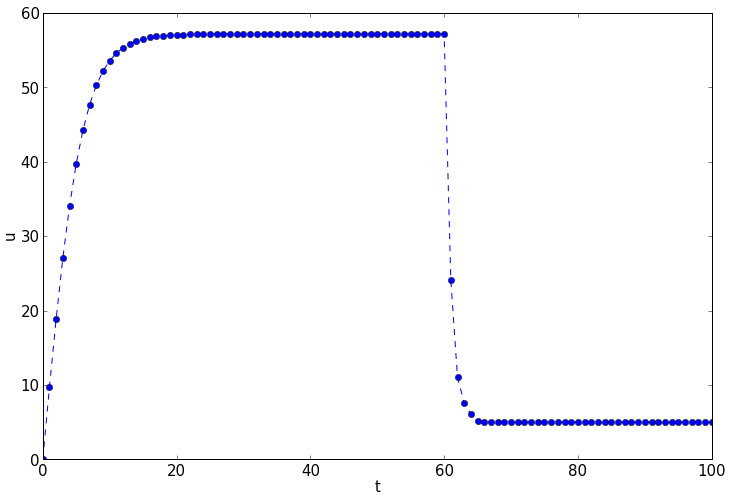
\includegraphics[max size={\textwidth}{\textheight}]{skydiving_files/skydiving_9_1.png}
    \par
    \end{center}
    
            \end{InvisibleVerbatim}
            
                \begin{InvisibleVerbatim}
                \vspace{-0.5\baselineskip}
    \begin{center}
    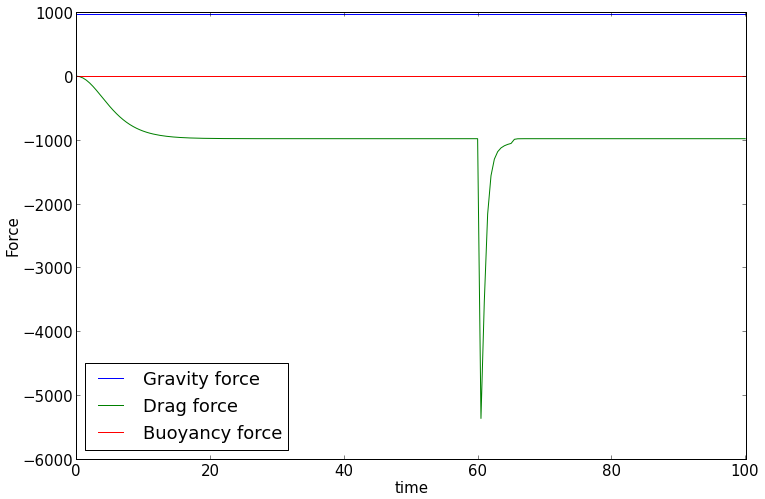
\includegraphics[max size={\textwidth}{\textheight}]{skydiving_files/skydiving_9_2.png}
    \par
    \end{center}
    
            \end{InvisibleVerbatim}
            
        
    
The first plot shows velocity as a function of time, while the second
one shows the various forces as a function of time. The terminal
velocity before the parachute opens is

    % Make sure that atleast 4 lines are below the HR
    \needspace{4\baselineskip}

    
        \vspace{6pt}
        \makebox[0.1\linewidth]{\smaller\hfill\tt\color{nbframe-in-prompt}In\hspace{4pt}{[}4{]}:\hspace{4pt}}\\*
        \vspace{-2.65\baselineskip}
        \begin{ColorVerbatim}
            \vspace{-0.7\baselineskip}
            \begin{Verbatim}[commandchars=\\\{\}]
\PY{n}{vt\PYZus{}freefall} \PY{o}{=} \PY{n}{u}\PY{o}{.}\PY{n}{max}\PY{p}{(}\PY{p}{)}
\PY{k}{print} \PY{l+s}{\PYZdq{}}\PY{l+s}{Terminal velocity before the parachute opens: }\PY{l+s}{\PYZdq{}}\PY{p}{,}\PY{n}{vt\PYZus{}freefall}
\end{Verbatim}

            
                \vspace{-0.2\baselineskip}
            
        \end{ColorVerbatim}
    

    

        % If the first block is an image, minipage the image.  Else
        % request a certain amount of space for the input text.
        \needspace{4\baselineskip}
        
        

            % Add document contents.
            
                \begin{InvisibleVerbatim}
                \vspace{-0.5\baselineskip}
\begin{alltt}Terminal velocity before the parachute opens:  57.1649254783
\end{alltt}

            \end{InvisibleVerbatim}
            
        
    
The terminal velocity after the parachute opens is

    % Make sure that atleast 4 lines are below the HR
    \needspace{4\baselineskip}

    
        \vspace{6pt}
        \makebox[0.1\linewidth]{\smaller\hfill\tt\color{nbframe-in-prompt}In\hspace{4pt}{[}5{]}:\hspace{4pt}}\\*
        \vspace{-2.65\baselineskip}
        \begin{ColorVerbatim}
            \vspace{-0.7\baselineskip}
            \begin{Verbatim}[commandchars=\\\{\}]
\PY{n}{vt\PYZus{}landing} \PY{o}{=} \PY{n}{u}\PY{p}{[}\PY{o}{\PYZhy{}}\PY{l+m+mi}{1}\PY{p}{]}
\PY{k}{print} \PY{l+s}{\PYZdq{}}\PY{l+s}{Terminal velocity after the parachute opens: }\PY{l+s}{\PYZdq{}}\PY{p}{,}\PY{n}{vt\PYZus{}landing}
\end{Verbatim}

            
                \vspace{-0.2\baselineskip}
            
        \end{ColorVerbatim}
    

    

        % If the first block is an image, minipage the image.  Else
        % request a certain amount of space for the input text.
        \needspace{4\baselineskip}
        
        

            % Add document contents.
            
                \begin{InvisibleVerbatim}
                \vspace{-0.5\baselineskip}
\begin{alltt}Terminal velocity after the parachute opens:  4.97556812654
\end{alltt}

            \end{InvisibleVerbatim}
            
        
    

        

        \renewcommand{\indexname}{Index}
        \printindex

    % End of document
    \end{document}


